% !TEX program = lualatex
% Generated by new_homework.sh — Math 113 Homework 3
\documentclass[11pt]{article}

\usepackage{fontspec}
\usepackage{microtype}
\usepackage{mathtools,amssymb,amsfonts,amsthm,bm}
\usepackage{enumitem}
\usepackage{booktabs,array,xcolor}
\usepackage{geometry,fancyhdr,setspace}
\usepackage{pdfpages}
\usepackage[hidelinks]{hyperref}
\usepackage[nameinlink,noabbrev]{cleveref}

% ---------- Page and paragraph rhythm (matches lecture/solutions templates) ----------
\geometry{margin=1in,headheight=15pt}
\setstretch{1.12}
\setlength{\parindent}{0pt}
\setlength{\parskip}{0.55em plus 0.12em minus 0.08em}
\setlength{\abovedisplayskip}{0.8em plus 0.2em minus 0.1em}
\setlength{\belowdisplayskip}{0.8em plus 0.2em minus 0.1em}
\allowdisplaybreaks[3]
\setlist{leftmargin=*,topsep=0.35em,itemsep=0.15em,parsep=0pt}

% ---------- Metadata ----------
\newcommand{\studentname}{Keshav Ramamurthy}
\newcommand{\coursename}{Math 113}
\newcommand{\courselongname}{Abstract Algebra}
\newcommand{\assignment}{Homework 3}
\newcommand{\term}{Fall 2026}

% ---------- Core notation (same as ~/.config/nvim/textemplate.tex) ----------
\newcommand{\N}{\mathbb{N}}
\newcommand{\Z}{\mathbb{Z}}
\newcommand{\Q}{\mathbb{Q}}
\newcommand{\R}{\mathbb{R}}
\newcommand{\C}{\mathbb{C}}
\newcommand{\F}{\mathbb{F}}
\newcommand{\K}{\mathbb{K}}
\newcommand{\E}{\mathbb{E}}
\newcommand{\Prob}{\mathbb{P}}
\newcommand{\1}{\mathbf{1}}
\newcommand{\eps}{\varepsilon}
\newcommand{\dd}{\,\mathrm{d}}
\newcommand{\abs}[1]{\left\lvert#1\right\rvert}
\newcommand{\norm}[1]{\left\lVert#1\right\rVert}
\newcommand{\ip}[2]{\left\langle#1,#2\right\rangle}
\newcommand{\set}[1]{\left\{#1\right\}}
\newcommand{\ceil}[1]{\left\lceil#1\right\rceil}
\newcommand{\floor}[1]{\left\lfloor#1\right\rfloor}
\newcommand{\given}{\,\middle\vert\,}
\newcommand{\indep}{\perp\!\!\!\perp}
\newcommand{\wh}[1]{\widehat{#1}}
\newcommand{\deriv}[2]{\frac{\mathrm{d}#1}{\mathrm{d}#2}}
\newcommand{\pderiv}[2]{\frac{\partial#1}{\partial#2}}
\newcommand{\lto}{\longrightarrow}
\newcommand{\st}{\text{ such that }}
\DeclareMathOperator{\Aut}{Aut}
\DeclareMathOperator{\End}{End}
\DeclareMathOperator{\Gal}{Gal}
\DeclareMathOperator{\Hom}{Hom}
\DeclareMathOperator{\Ker}{ker}
\DeclareMathOperator{\im}{im}
\DeclareMathOperator{\rank}{rank}
\DeclareMathOperator{\nullity}{nullity}
\DeclareMathOperator{\Span}{span}
\DeclareMathOperator{\tr}{tr}
\DeclareMathOperator{\diag}{diag}
\DeclareMathOperator{\spec}{spec}
\DeclareMathOperator{\ord}{ord}
\DeclareMathOperator{\supp}{supp}
\DeclareMathOperator{\diam}{diam}
\DeclareMathOperator{\Var}{Var}
\DeclareMathOperator{\Cov}{Cov}
\DeclareMathOperator*{\argmin}{arg\,min}
\DeclareMathOperator*{\argmax}{arg\,max}

% ---------- Statement environments ----------
\newtheorem{problem}{Problem}
\newtheorem{theorem}{Theorem}
\newtheorem{lemma}{Lemma}
\newtheorem{proposition}{Proposition}
\newtheorem{corollary}{Corollary}
\theoremstyle{definition}
\newtheorem{definition}{Definition}
\newtheorem{example}{Example}
\newtheorem{remark}{Remark}

% ---------- Solution machinery (matches solutions.tex / textemplate.tex) ----------
\newenvironment{solution}{\begin{proof}[Solution]}{\end{proof}}
\newenvironment{answer}{\begin{proof}[Answer]}{\end{proof}}
\renewcommand{\qedsymbol}{$\square$}
\newcommand{\exercise}[1]{%
  \par\goodbreak\medskip\noindent\textbf{Exercise #1}\par\nopagebreak\smallskip\nopagebreak}
\newcommand{\exref}[1]{\textsf{\textbf{Exercise~#1}}}
\newenvironment{claim}{\par\smallskip\noindent\textit{Claim.}\ }{\par\smallskip}
\newenvironment{idea}{\par\smallskip\noindent\textit{Idea.}\ }{\par\smallskip}
\newenvironment{proofsketch}{\par\smallskip\noindent\textit{Proof sketch.}\ }{\par\smallskip}

% ---------- Header ----------
\pagestyle{fancy}
\fancyhf{}
\fancyhead[L]{\coursename}
\fancyhead[C]{\assignment\ — my solutions}
\fancyhead[R]{\studentname}
\fancyfoot[C]{\thepage}

\begin{document}

% ---------- Title ----------
\begin{center}
  {\Large\sffamily\bfseries \coursename\ -- \courselongname}\par\vspace{3pt}
  {\sffamily \assignment\ — my solutions}\par\vspace{3pt}
  {\small\sffamily \term\quad\textbullet\quad \studentname}
\end{center}
\medskip
\hrule
\bigskip

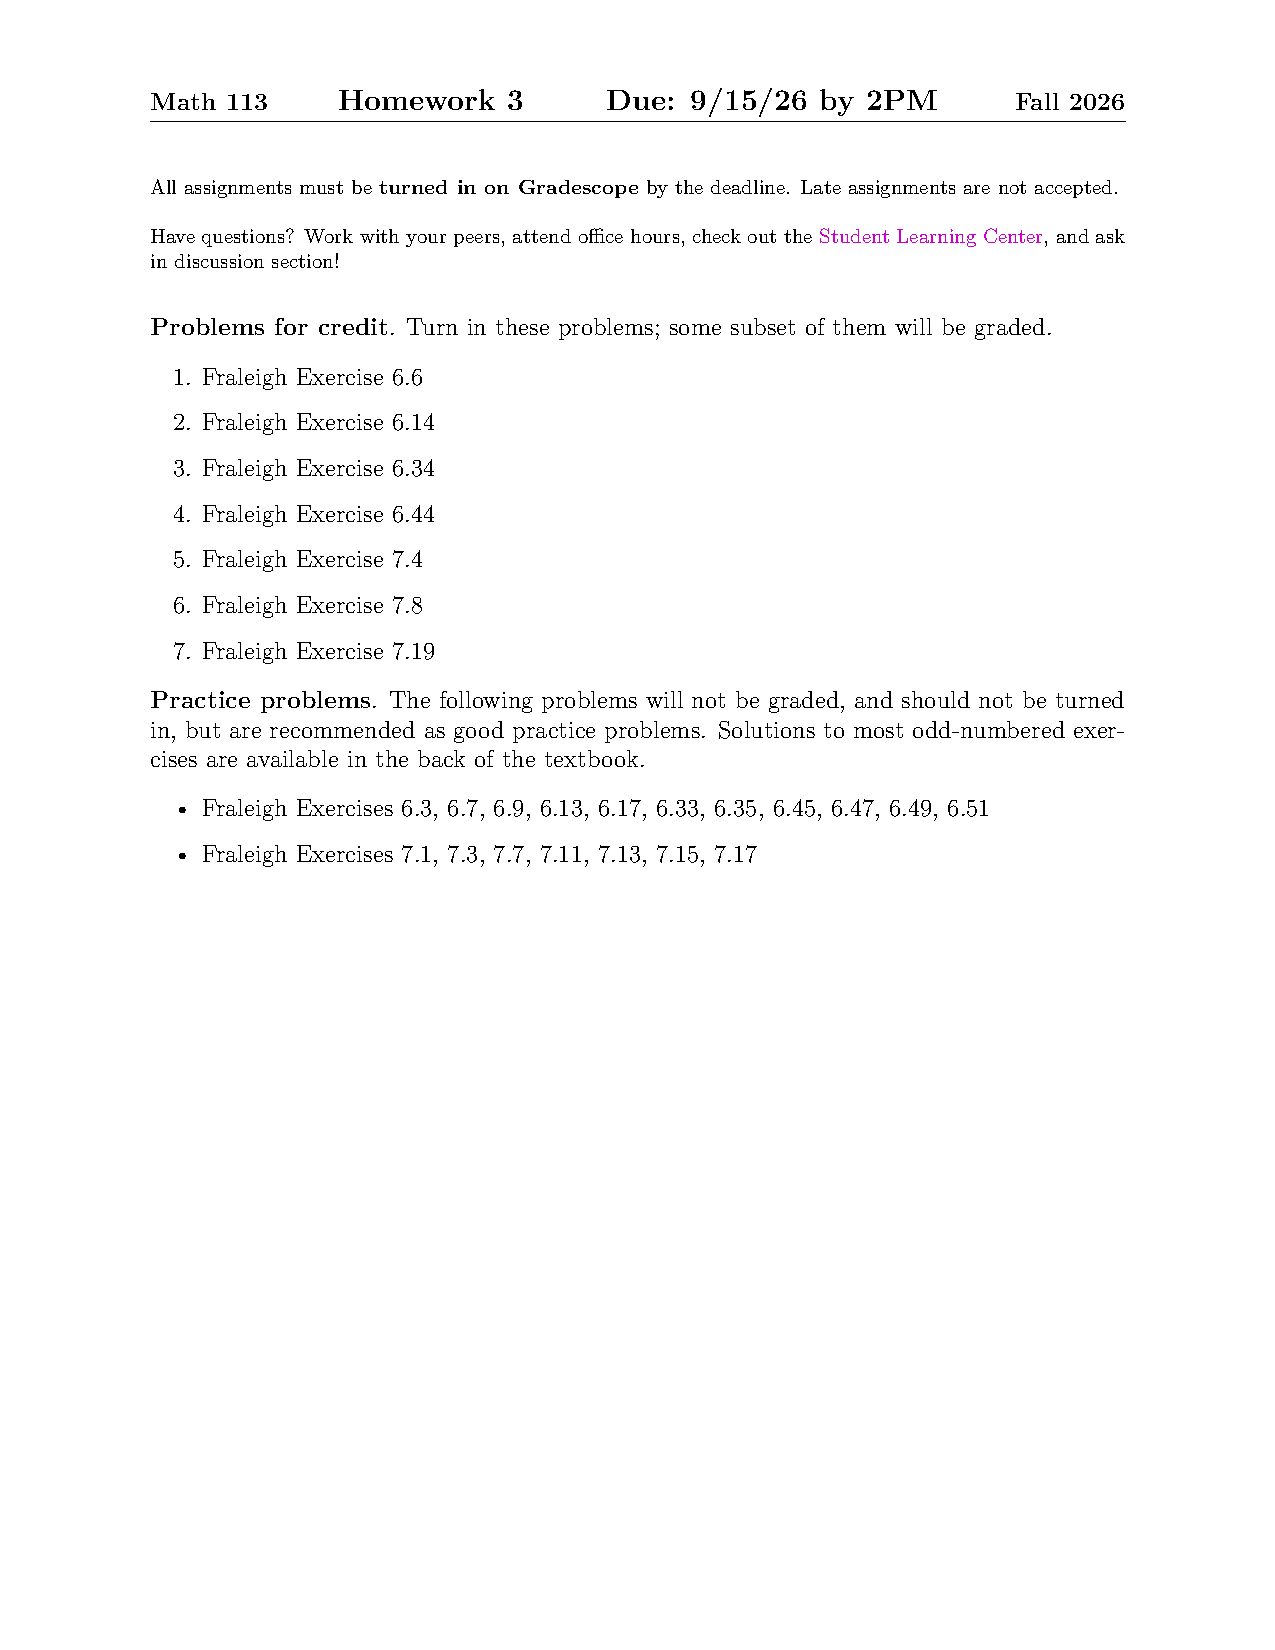
\includepdf[pages=-,pagecommand={\thispagestyle{empty}}]{hw3.pdf}
\clearpage

\section*{Solutions}
\subsubsection*{Problem 1 (Fraleigh Exercise 6.6)}
\begin{solution}
    $\gcd(48, 88) = 8$ as $48 = 8 \cdot 6, 88 = 8 \cdot 11$ and 8 and 11 are relatively
    prime.
% Write your proof, calculation, or argument here.
\end{solution}
\subsubsection*{Problem 2 (Fraleigh Exercise 6.14)}
\begin{solution}
    On $\mathbb{Z}_8$, we are examining functions $f : G \rightarrow G$ that satisfies $$x, y \in G,  f(x + y) = f(x) + f(y)$$
    Notice for $\mathbb{Z}_8$, $\mathbb{Z} = \langle 1 \rangle$
    So we want to find the number of generators $\langle g \rangle$ that can generate
    $\mathbb{Z}_8.$
\par    Let's examine what other values can be generators. Suppose $G = \langle k
\rangle $ for $k\ne 1.$
\par  This would generate $0, k, 2k, \cdots$ modulo 8.
\par This would not generate the entire residue class mod 8 if $nk$ reaches $0$ 
\par This is because notice if $nk = 0$ has a solution, then $nk\equiv1 \mod 8$ would not
have a solution, meaning not all values would be hit.
\par The residues relatively prime to $8$ are $1, 3, 5, 7$ so the answer is 4.
% Write your proof, calculation, or argument here.
\end{solution}
\subsubsection*{Problem 3 (Fraleigh Exercise 6.34)}
\begin{solution}
We attempt to find an example of an infinite group that is not cyclic. Every infinite
cyclic group must be isomorphic to $\langle Z, +\rangle$
\par Consider $G = \{Q \setminus \{0\}, *\}$ Let's first examine if its a group.
\par It has a identity 1, and notice the inverse for $a \in Q \setminus\{0\}$
is $\frac{1}{a}.$
\par Closure also holds as $p, q \in Q \setminus \{0\}$, $pq \in Q\setminus\{0\}$
\par We have to show that this group is not cyclic. For sake of contradiction, suppose
there exists a generator for this group $\langle k\rangle$
Consider arbitrarily $2$ and $3$, we'd have $$\exists n, m \in \mathbb{Z}^{+} \text{ s.t
} k^n = 2, k^m = 3$$
Notice, we'd have $(k^n)^m = 2^m, (k^m)^n = 3^n \rightarrow 2^m = 3^n$ which is a
contradiction as $n$ and $m$ are positive integers (this only holds for $m = n  = 0.$)
% Write your proof, calculation, or argument here.
\end{solution}
\subsubsection*{Problem 4 (Fraleigh Exercise 6.44)}
\begin{solution}
We have a cyclic group $G$ with generator $a$ and $G'$ a group such that $G \cong G'$
\par We have a function $\phi: G \rightarrow G'.$ and we wish to show that $\phi(x)$ is
completely determined by the value $\phi(a).$ So if two isomorphisms have the same value
at a, we wish to show they are the same function.
\par Notice we can write the inputs as $\phi(a^1) = \varphi(a^1)  = b$ for some $b \in G'$
\par And we wish to basically show that this implies $\phi(a^i) = \varphi(a^i)$ for all
i (on Z)
We first consider the homomorphism property on $\phi$: $$\phi(x * y) = \phi(a^{i + j})
= \phi(a^{i})\phi(a^{j})$$ where here $x = a^i, y = a^j.$
Notice this creates $$\phi(a^{2}) = \phi(a)\phi(a) = \phi(a)^2$$ and similarly
$\phi(a^i) = \phi(a)^i.$ (and holds for negatives because homomorphism preserves
inverses)
Notice this applies analogously to $\varphi$, so $\varphi(a^{i}) = \varphi(a)^i.$
Thus, we are done, as any $$\forall x \in G,\exists i \in \mathbb{Z},  a^{i} = x
\rightarrow \phi(a^i) = \varphi(a^i) = \phi(a)^i = \varphi(a)^i \text{ and } \phi(a) =
\varphi(a) \text{ as given }$$
so for all values of x, these are the same.
% \par So given that $a$ is a generator, using the property of homomorphism: 
% \par Consider an arbitrary $\phi(x) = y.$

% Write your proof, calculation, or argument here.
\end{solution}
\subsubsection*{Problem 5 (Fraleigh Exercise 7.4)}
\begin{solution}
    The elements of the subgroup generated by $\{12, 30\}$ of $\mathbb{Z}_{36}$
\par    We first consider the values $12k$ attains mod 36, and we can pretty easily see
that it goes $0, 12, 24, 0, \cdots.$
\par For 30, it goes $0, 30, 24, 18, 12, 6, 0, \cdots$ 
\par So the subgroup of $\mathbb{Z}_{36}$ is $\{0, 6, 12, 18, 24, 30\}$ or just the subgroup
with generator 6.
% Write your proof, calculation, or argument here.
\end{solution}
\subsubsection*{Problem 6 (Fraleigh Exercise 7.8)}
\begin{solution}
We start at $a^2b$ in the diagram. \par Each subsequent multiplication by a we go around
following the arrows. \par So $(a^2b) a$ is $ab$, $(a^2b)a^2 = b$, and finally $a^2b(a^3) =
a^3b$ which is our answer.
% Write your proof, calculation, or argument here.
\end{solution}
\subsubsection*{Problem 7 (Fraleigh Exercise 7.19)}
\begin{solution}
    We wish to show the existence of a non abelian group of size $2n$ for $n \ge 3$
    generated by two elements of order 2.

\par    Consider the first where on $(1, 2, \cdots, n)$ you keep 1 as a fixed point
and reverse $(2, \cdots, n)$
    \par Now consider the second manipulation that reverses the entire permutation, so $$(1, 2, \cdots, n) \rightarrow (n, n-1, n-2, \cdots, 1) \rightarrow (1, 2,\cdots, n)$$
    Consider applying both operations, and examining position one.
\par    Let's track 1 first, then examine the rest. $ 1\rightarrow 1 \rightarrow n \rightarrow 2 \rightarrow n - 1 \rightarrow 3 \rightarrow n - 3 \rightarrow 4 \rightarrow n - 4 \cdots $
\par So it seems like it generates all $2n$ and we'll show it rigorously.
\par Let the first be defined by a function $A$ where $A(1) = 1$ and $A(i) = n + 2 - i$ for
$n \ge i \ge 2.$
\par And let's define the second as $B(i) = n + 1 - i$ for $n \ge i \ge 1$
$B(A(1)) = n.$
\par And, $T = B(A(i))$ for $i \ge 2$ is $B(n + 2 - i) = (n + 1) - (n + 2 - i) = i - 1.$
So thus, $1 \rightarrow n \rightarrow n - 1\rightarrow \cdots \rightarrow 2$ hits all n
elements.
\par We can generate another $n$ by applying A after all the terms above(which are
distinct for the same idea, they enumerate them all in order).
\par To show that this creates $2n$ distinct elements, we consider the function on 2,
and for sake of contradiction assume $T^{i} A(2) = T^{j} (2)$
$$A(2) = n\rightarrow T^i (A(2)) = T^{i+1}(n)$$
% Yet notice that $T(1) = n$, so we have $T^{i} A(2) = T^{i + 1} (1)$
% we could also write $2$ as $T^{n-1}(1)$ so we'd have 
Now let's manipulate $T^j(2).$ We get $2 = T^{n-1}(1)$ so $T^j(2) = T^{j + n - 1}(2) $
$$T^{i+1}(n) = T^{j + n - 1}(n)$$
   Since powers of $T$ were distinct with order n, setting the exponents equal modulo n
   yields $$i + 1 \equiv j + n - 1 \mod n \rightarrow i - j \equiv -2 \mod n$$

Now, to finish up, let's apply this back onto 1.
\par On 1, we'd have $$T^{i} A(1) = T^{j} (1)\rightarrow T^{i} (1) = T^{j}(1)$$ because
$A(1) = 1$, and this yields $i \equiv j \mod n$, which is a contradiction, so there must
be $2n$ distinct elements.
\par Now, let's show that it isn't abelian.
% We consider $B \circ A$ and now let's consider $A \circ B$
% For 1, we have $A(B(1)) = A(n) = 2.$
% \par And for $n \ge i \ge 2$, we have $A(B(i)) = A(n + 1 - i) = (n + 2) - (n + 1 - i) =
% i + 1$
% so, this cycles, but $1 \rightarrow 2 \rightarrow 3\cdots\rightarrow n$
% write your proof, calculation, or argument here.
\par Notice we showed $B \circ A$ has order $n \ge 3$, and for sake of contradiction suppose
$G$ is abelian.
\par Then, we have that $B \circ A = A \circ B$ and $(BA)^2 = BABA = BB AA$ and since these
are both order two, this would mean that this would be the identity or permute back in
this case, which is a contradiction, as this would imply an order less than 3.
\end{solution}

\end{document}
